\documentclass[14pt]{article}

\usepackage[letterpaper,margin=0.75in]{geometry}
\setlength{\parindent}{0pt}

\usepackage{amsmath}
\usepackage{booktabs}
\usepackage{fancyhdr}
\usepackage{standalone}
\usepackage{csvsimple}
\usepackage{float}
\usepackage{csvsimple}
\usepackage{hyperref}
\usepackage{biblatex} %Imports biblatex package
\usepackage{minted} % For matlab code highlighting

% Bibliography
\addbibresource{all.bib}

% \include{data/reaction-time.csv}

\pagestyle{fancy}


\begin{document}


\title{The physics of light sails}
\date{}



\author{Sidney Pauly}
\def\theuoastudentid{52104132}

\makeatletter

\let\thetitle\@title
\let\theauthor\@author
\let\thedate\@date


\makeatother




\fancyhf{}
\fancyhead[L]{Name: \theauthor}
% \fancyhead[C]{}
\fancyhead[R]{ID: \theuoastudentid}


% \maketitle

\begin{titlepage}
  \begin{center}
    \Large
    \textbf{\thetitle}
        
    \vspace{0.4cm}
    \large
    PX2013 - Essay
        
    \vspace{0.4cm}
    \textbf{\theauthor}\\
    \textbf{\theuoastudentid}

       
    \vspace{0.9cm}
    \textbf{Abstract}
    \end{center}
    Light sails are an alternative way to propel spacecraft. Their main advantage over other propulsion
    methods is that they do not require any fuel to operate and are therefore not limited by the same constraints
    as conventional propulsion systems.
    An overview of the base physics enabling this propulsion system is outlined. Specific focus lies on the
    the optical properties of such sails and how they impact the efficiency of the sail. 
    A new computational model based on these physical behavior is introduced. It is then tested
    on a specific sail to calculate the sail's efficiency.

  \vfill

  \begin{center}

    University of Aberdeen\\
    Scotland\\
    UK\\
    \thedate
    \vspace{0.4cm}
    \url{https://github.com/sidney-pauly/papers}
  \end{center}
\end{titlepage}

\section{Introduction}
Conventional propulsion systems for space craft face a fundamental challenge. 
In space, there is nothing to push off to gain momentum. As such spacecraft have to carry their
own mass, that can be ejected as exhaust, which then propels the spacecraft forwards. For every kilo
of fuel that is brought along, even more fuel has to be brought to propel that fuel. This results in
diminishing returns and therefore poses a limit on the maximum delta-v\footnote{Delta-v denotes the change in velocity.
It is the primary measure for the usefulness of any propulsion system in space. This is because to get to other places in space,
a craft needs to change its orbit, which in turn means changing the velocity} that can be delivered through
such a system\autocite{dunbar}.\\
\\
Light sails are one of the few propulsion methods, which don't face this problem. Light sails are essentially big mirrors that reflect
light. As photons carry momentum, reflecting them leads to an opposite force applied to the spacecraft.

\begin{figure}[H]
  \centering
  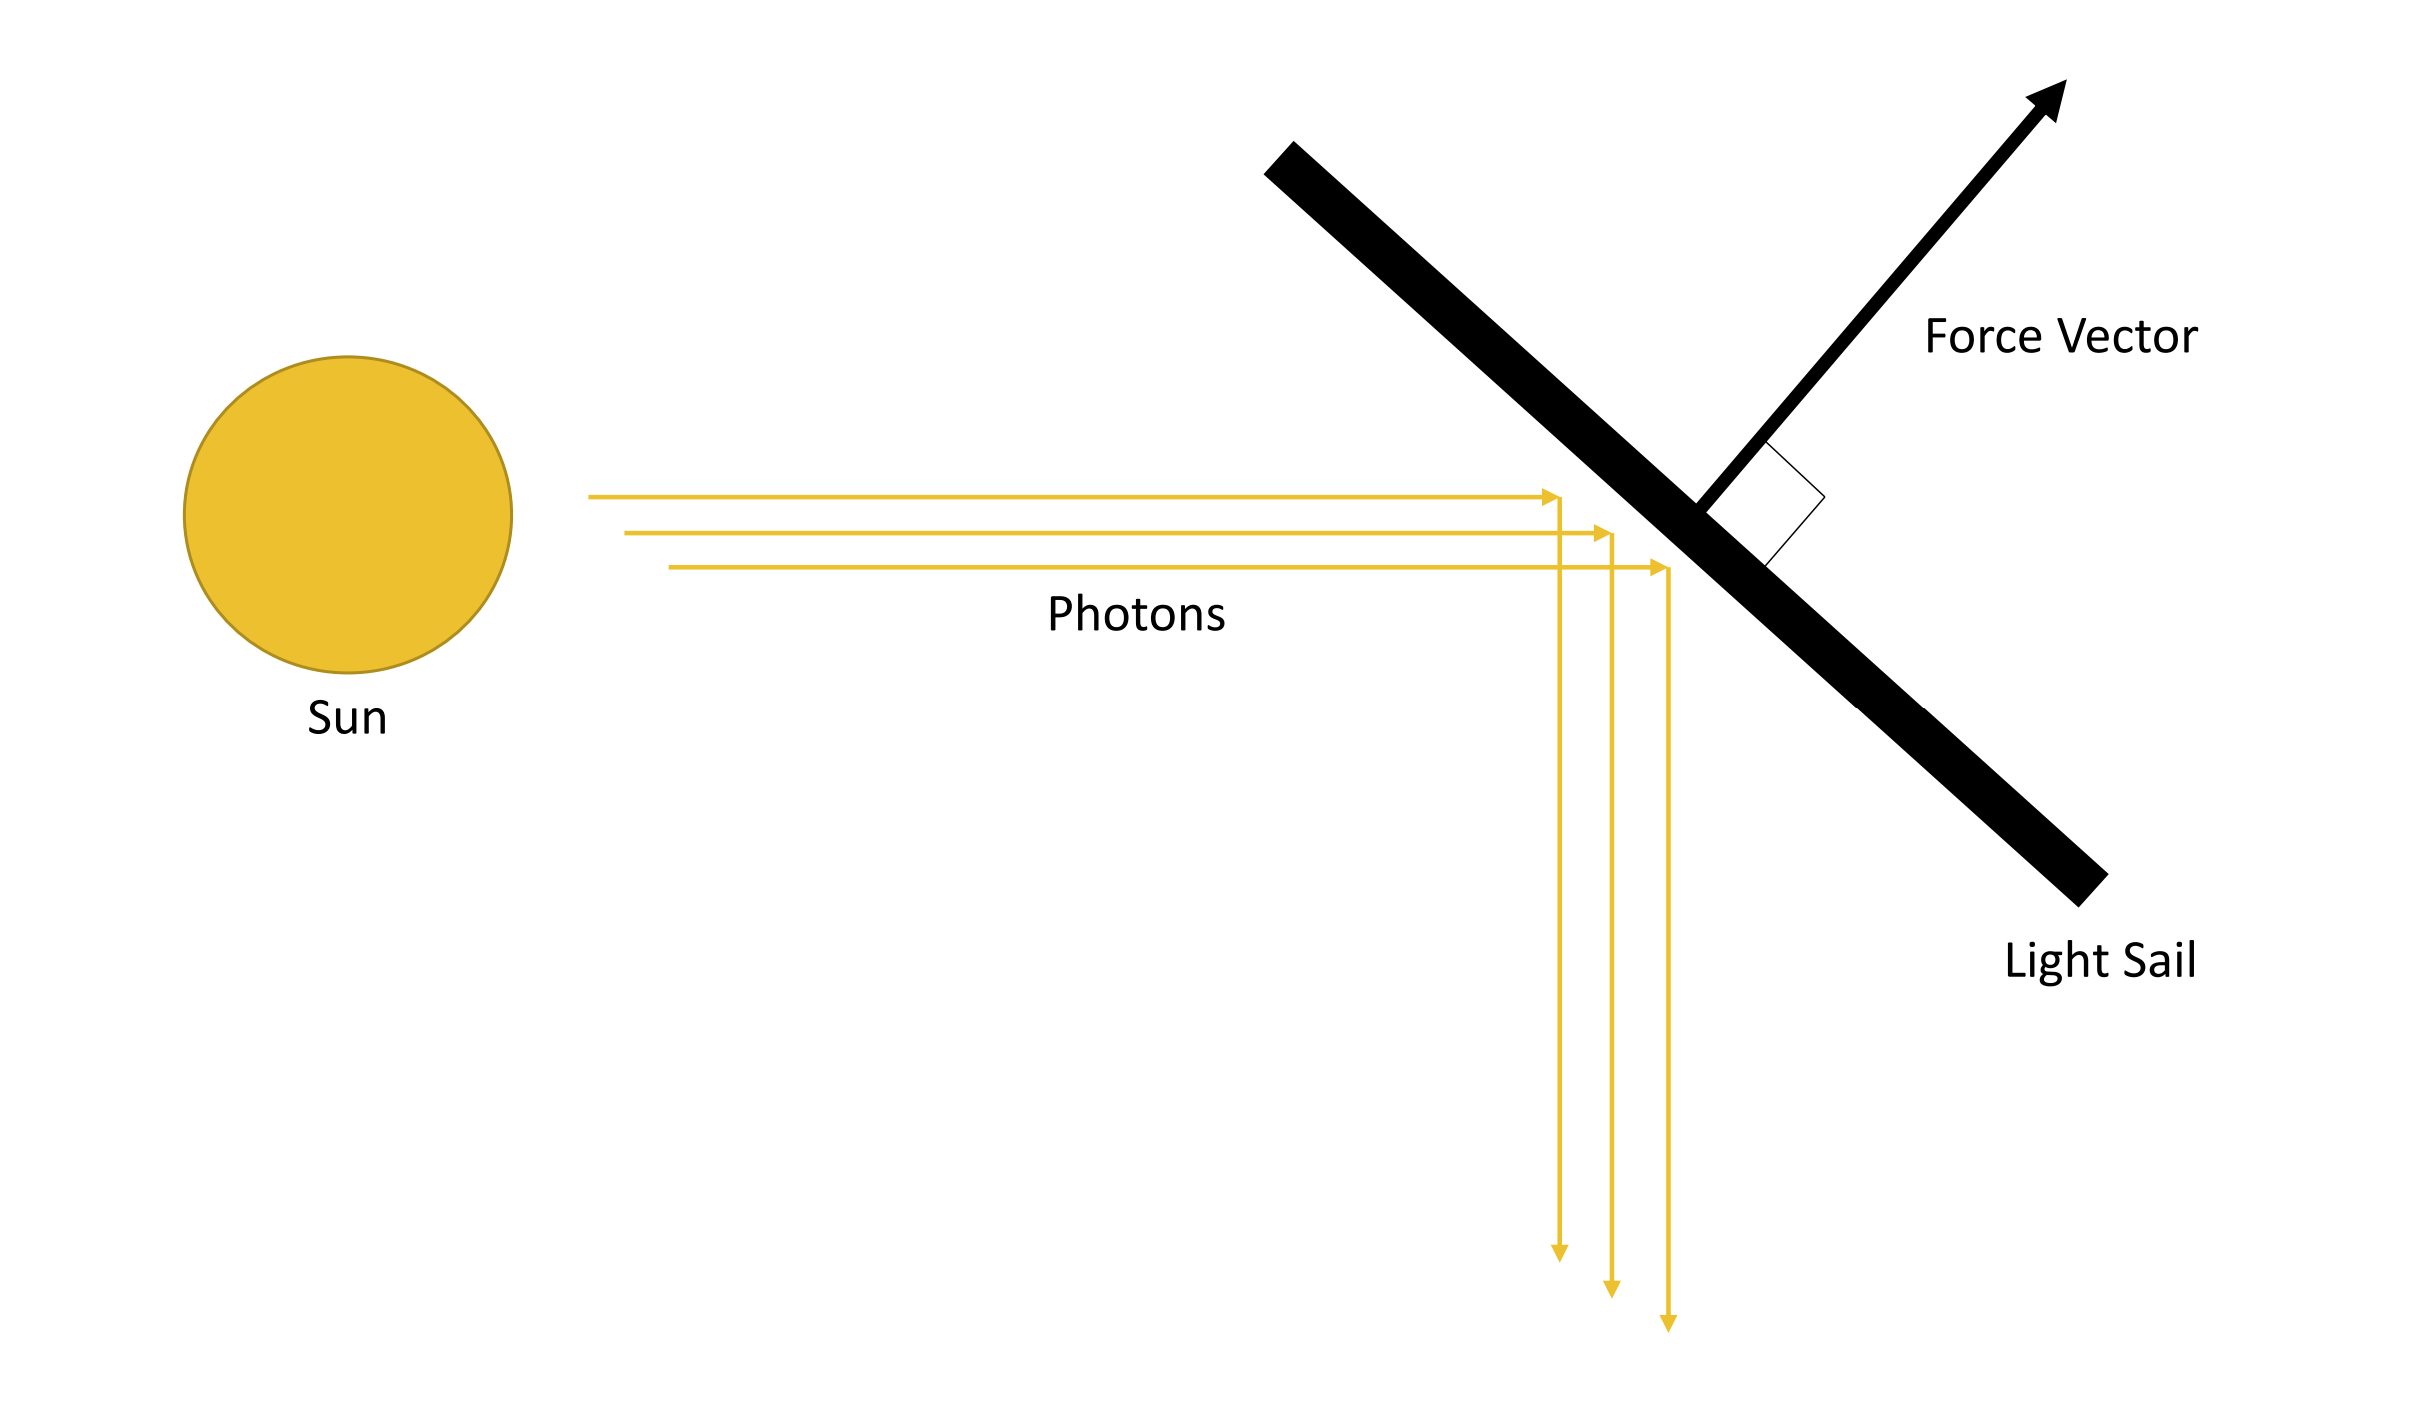
\includegraphics[width=14cm]{./resources/solar_sail.png}
  \caption{Basic principle behind a light sail}
  \label{fig:sail_principle}
\end{figure}

As this does not consume any fuel (or even any other type of power), the spacecraft can in theory gain any amount of delta-v given enough time.

\section{Basic physical principles}

\subsection{Momentum of a photon}

Even though photons do not have any mass, they have momentum. That photons have momentum is a consequence of general relativity\autocite{openstax},
however as this essay is focused on optics, no further explanation will be given. The momentum of a single photon is given by:

\begin{equation}
  p = \frac{h}{\lambda}
  \label{eq:light_momentum}
\end{equation}

Important to the design of a light sail, is that the momentum ($p$) is inversely proportional to the wavelength. This means that for a light
sail to be effective it has reflect or absorb a high percentage of these high energy photons.

\subsection{Momentum transfer}

In order to later determine the actual efficiency of any given light sail, it makes sense to look at the three base forces that can
be applied by light on the sail:

\begin{enumerate}
  \item The light is perfectly reflected off the sail's surface
  \item The light is perfectly absorbed by the sail
  \item The sail emits light through blackbody radiation
\end{enumerate}

Perfect reflection and perfect absorption can be modeled as completely elastic and inelastic collisions respectively\autocite{paschotta}.
In case of the photons being perfectly reflected, the inverse of a photons momentum change will be applied to the sail
(perfect elastic collision).

\begin{figure}[H]
  \centering
  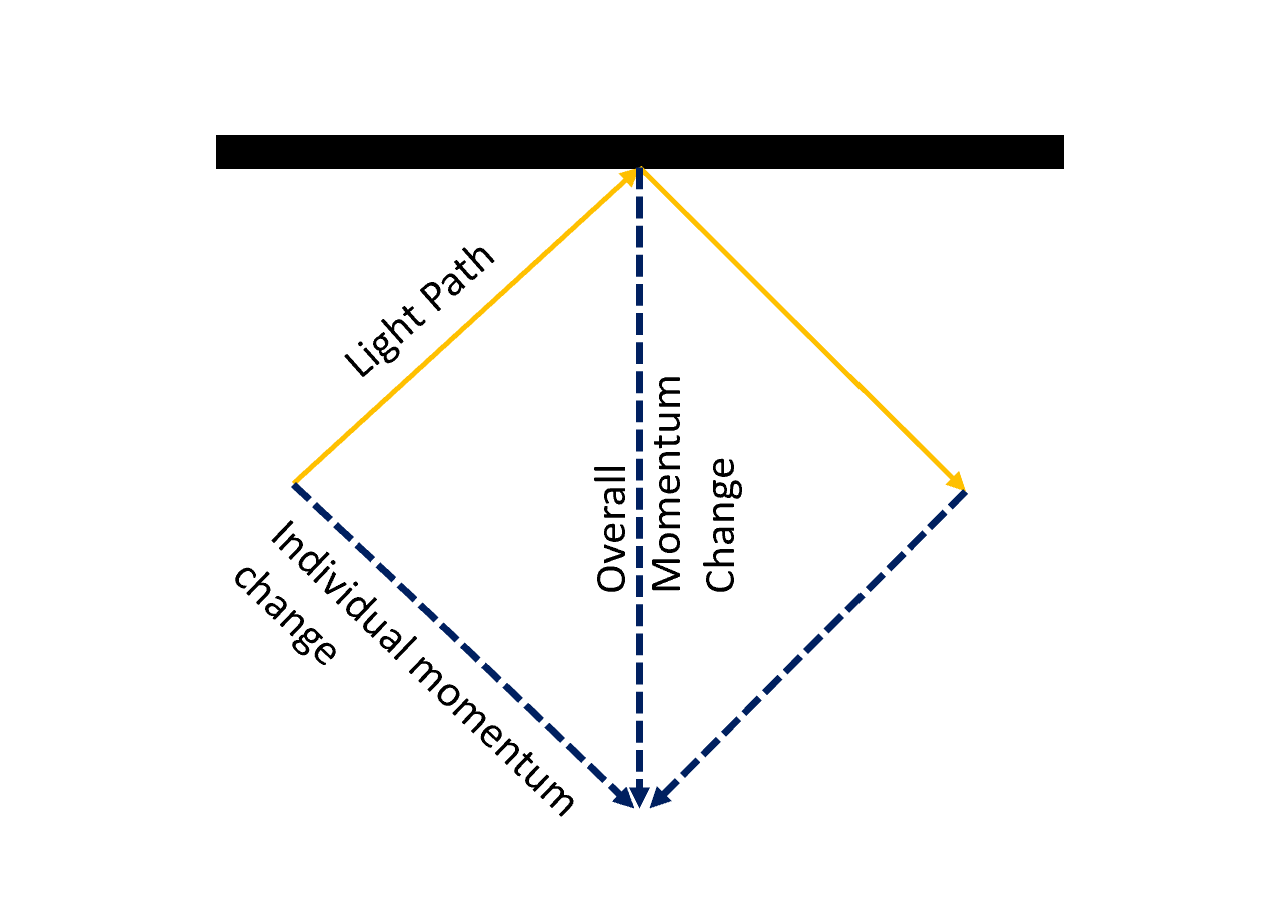
\includegraphics[width=14cm]{./resources/solar_sail_momentum.png}
  \caption{Momentum transfer assuming perfect reflection}
  \label{fig:sail_momentum_reflected}
\end{figure}

The net momentum transferred will be twice the momentum normal to the sail.
This is because the parallel component cancels out (figure \ref{fig:sail_momentum_reflected}).

If the photon is absorbed, all of the momentum that the photon previously carried by the photon is transferred to
the sail (perfect inelastic collision). If the sail is not aligned with the light this can lead to a force component
parallel to the sails surface.\\
\\
The case of emission is the inverse of absorption. Instead of the sail gaining the momentum of the photon, it gains the inverse. 
Emission of blackbody radiation will happen in all directions. If all surfaces of the sail have the same geometry,
temperature and emission characteristics, the blackbody radiation will lead to no net force.

\begin{figure}[H]
  \centering
  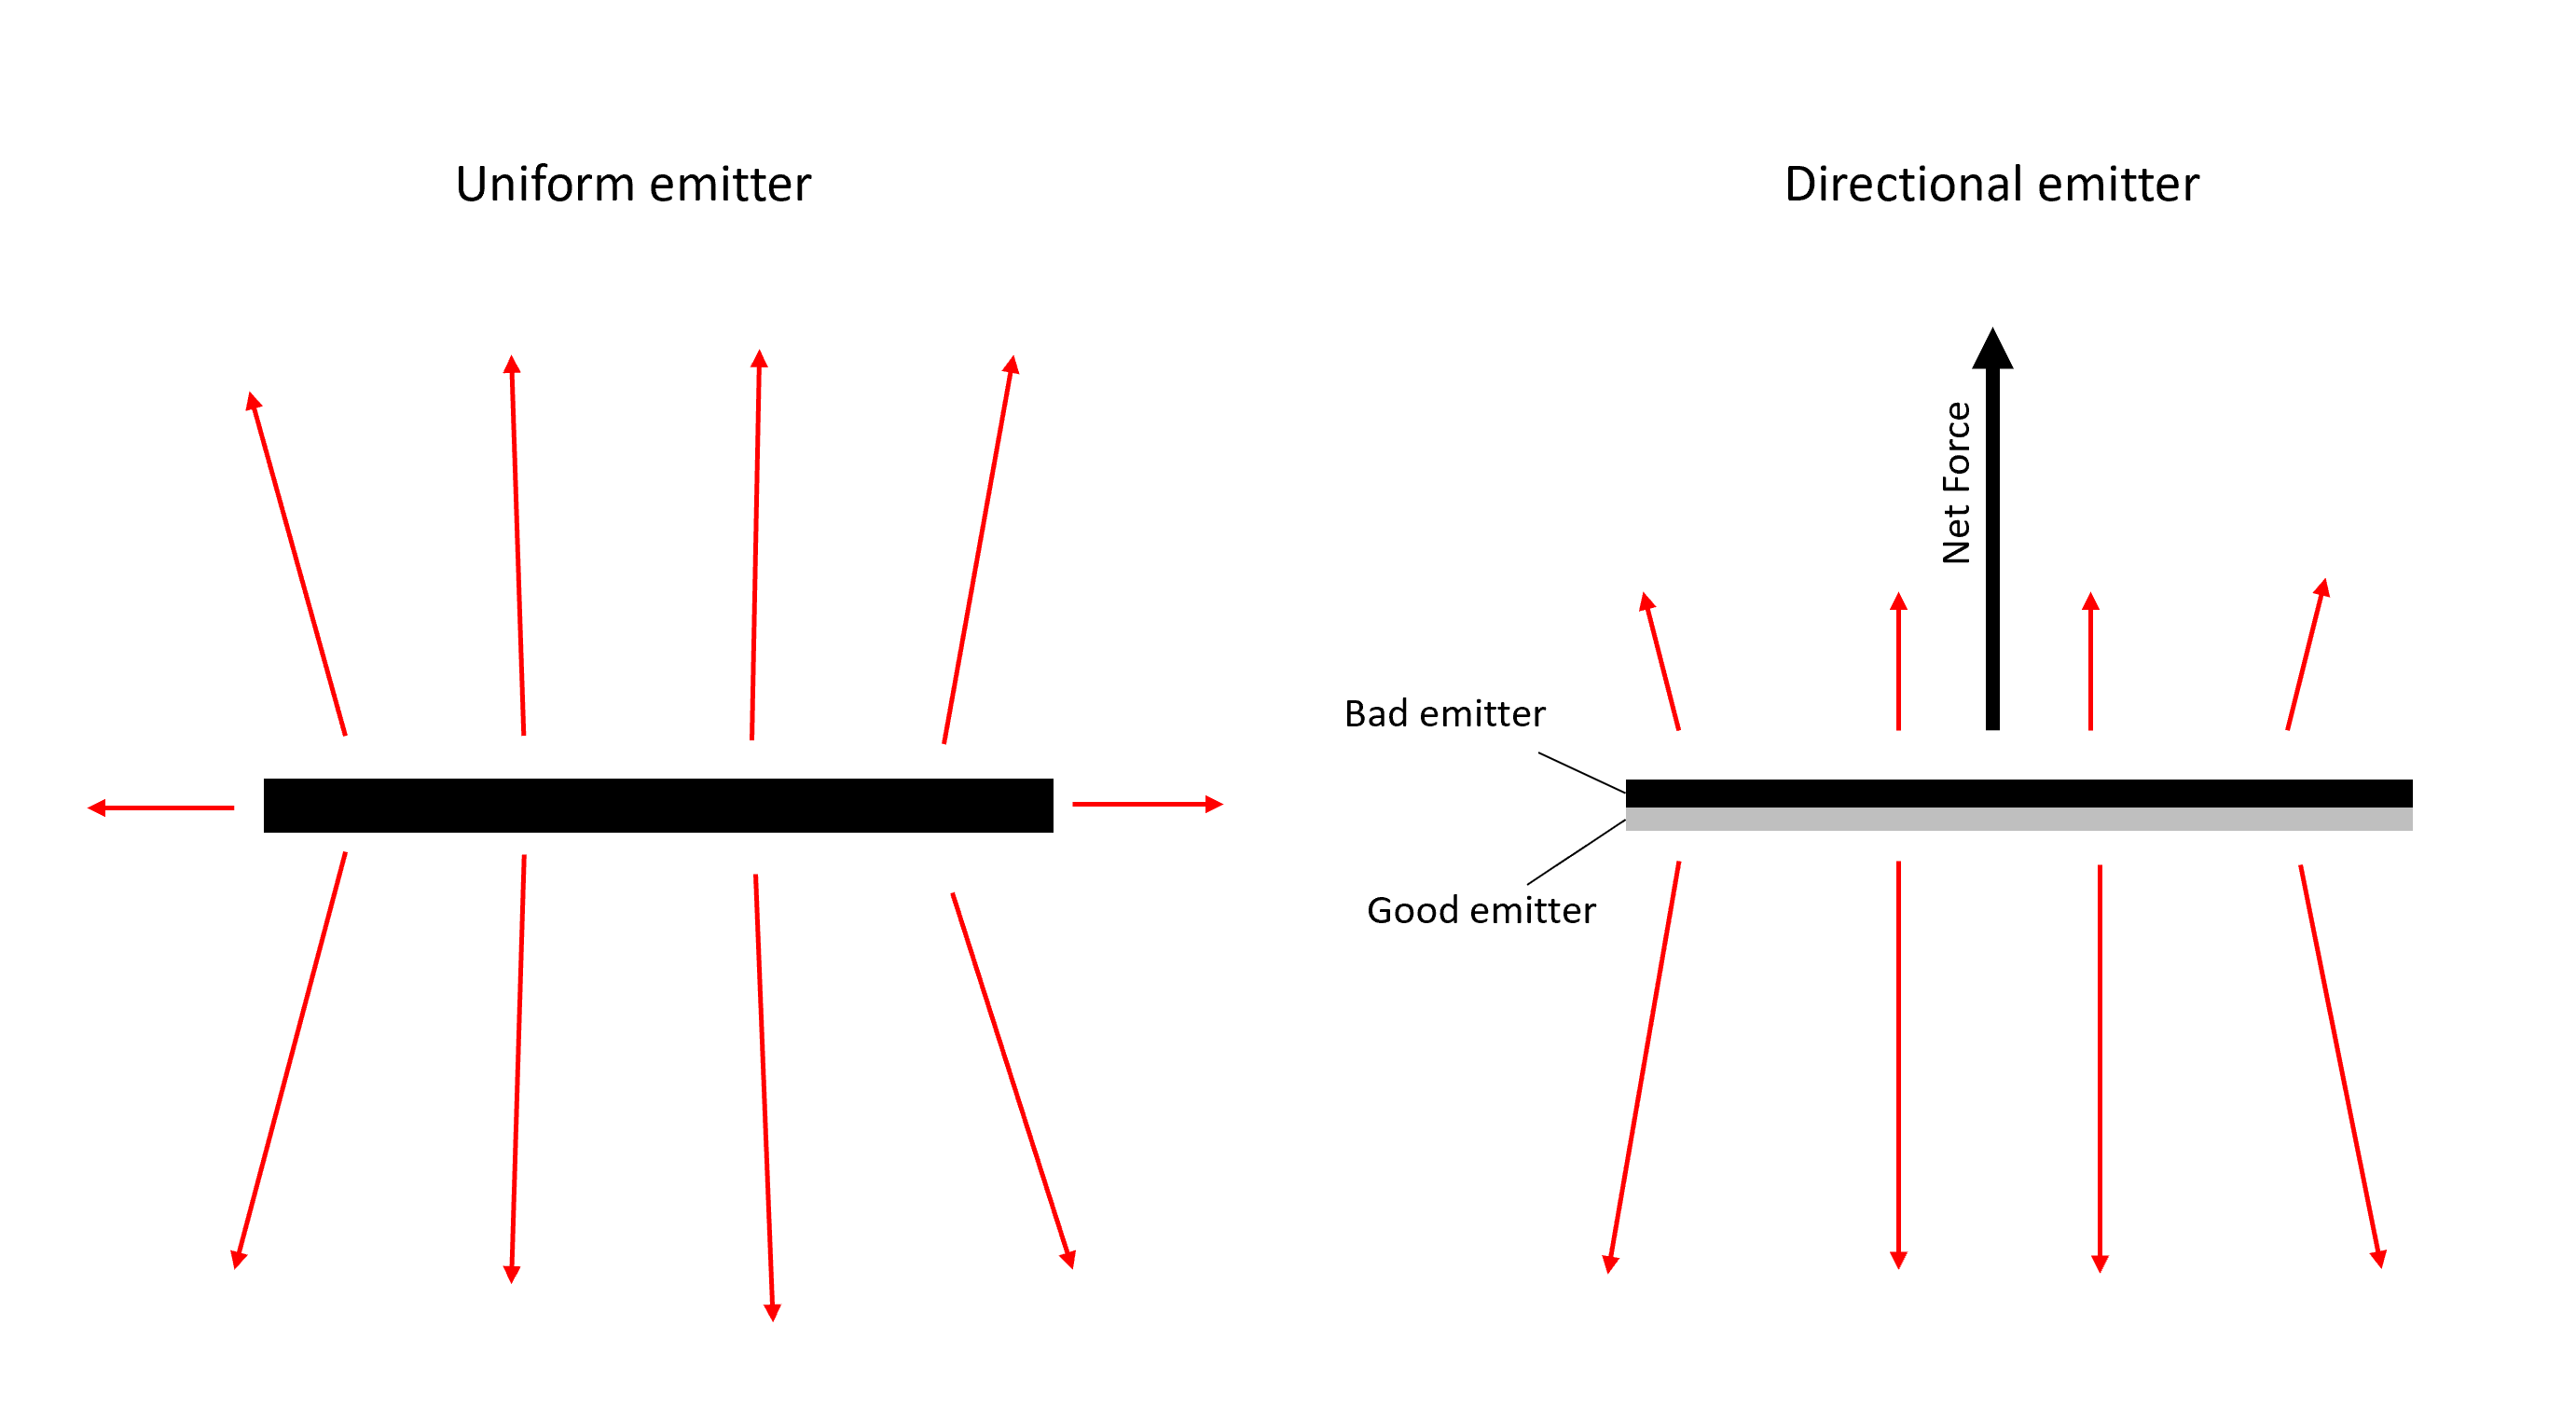
\includegraphics[width=14cm]{./resources/dicrectional_emitter.png}
  \caption{Uniform vs. none uniform emitter}
  \label{fig:dicrectional_emitter}
\end{figure}

To make a light sail even more efficient, it is desireable to have more photons emitted in the direction of the light source, as this creates an additional net force in the
direction of the absorption and reflection forces (figure \ref{fig:dicrectional_emitter}). To achieve this, one of the surfaces needs to emit less blackbody radiation than
the other. This can either be achieved by having a less emissive material on that side of the sail or by having a temperature gradient between the two sides (higher temperature
leads to more energy emitted).\\

Assuming perfect reflection of all light and an angle of incidence $\theta_i = 0^\circ$ a formula for a 100\% efficient sail can be derived
by putting together \ref{eq:light_momentum} with newtons 2nd law $F = \frac{dp}{dt}$ as well as the formula for the energy of a photon $ E = h \frac{\lambda}{c}$:

\begin{equation}
  F = \frac{dE}{dt} * \frac{1}{c} = \frac{P}{c}
  \label{eq:light_force}
\end{equation}

If the light is reflected rather than absorbed this force needs to be multiplied as detailed.


\section{Complications}

In a real sail, these forces combine to produce the net force of the sail. Crucial to the analysis is that all the absorbed radiation eventually gets emitted again
by the sail (as soon as it reaches a stable temperature). This means that if the sail has bad reflectivity (reflects a low percentage of light), absorption and
emission characteristics become more important.\\
\\
Furthermore, a sail should be as light as possible to get the most acceleration out of the generated force. A design out of a thin structural base layer made out
of a high strength material such as kevlar, carbon fibre or similar, coated with desirable optical layers is suited best. In turn that means that the interactions
of the light with the sail get quite complex.\\

\begin{figure}[H]
  \centering
  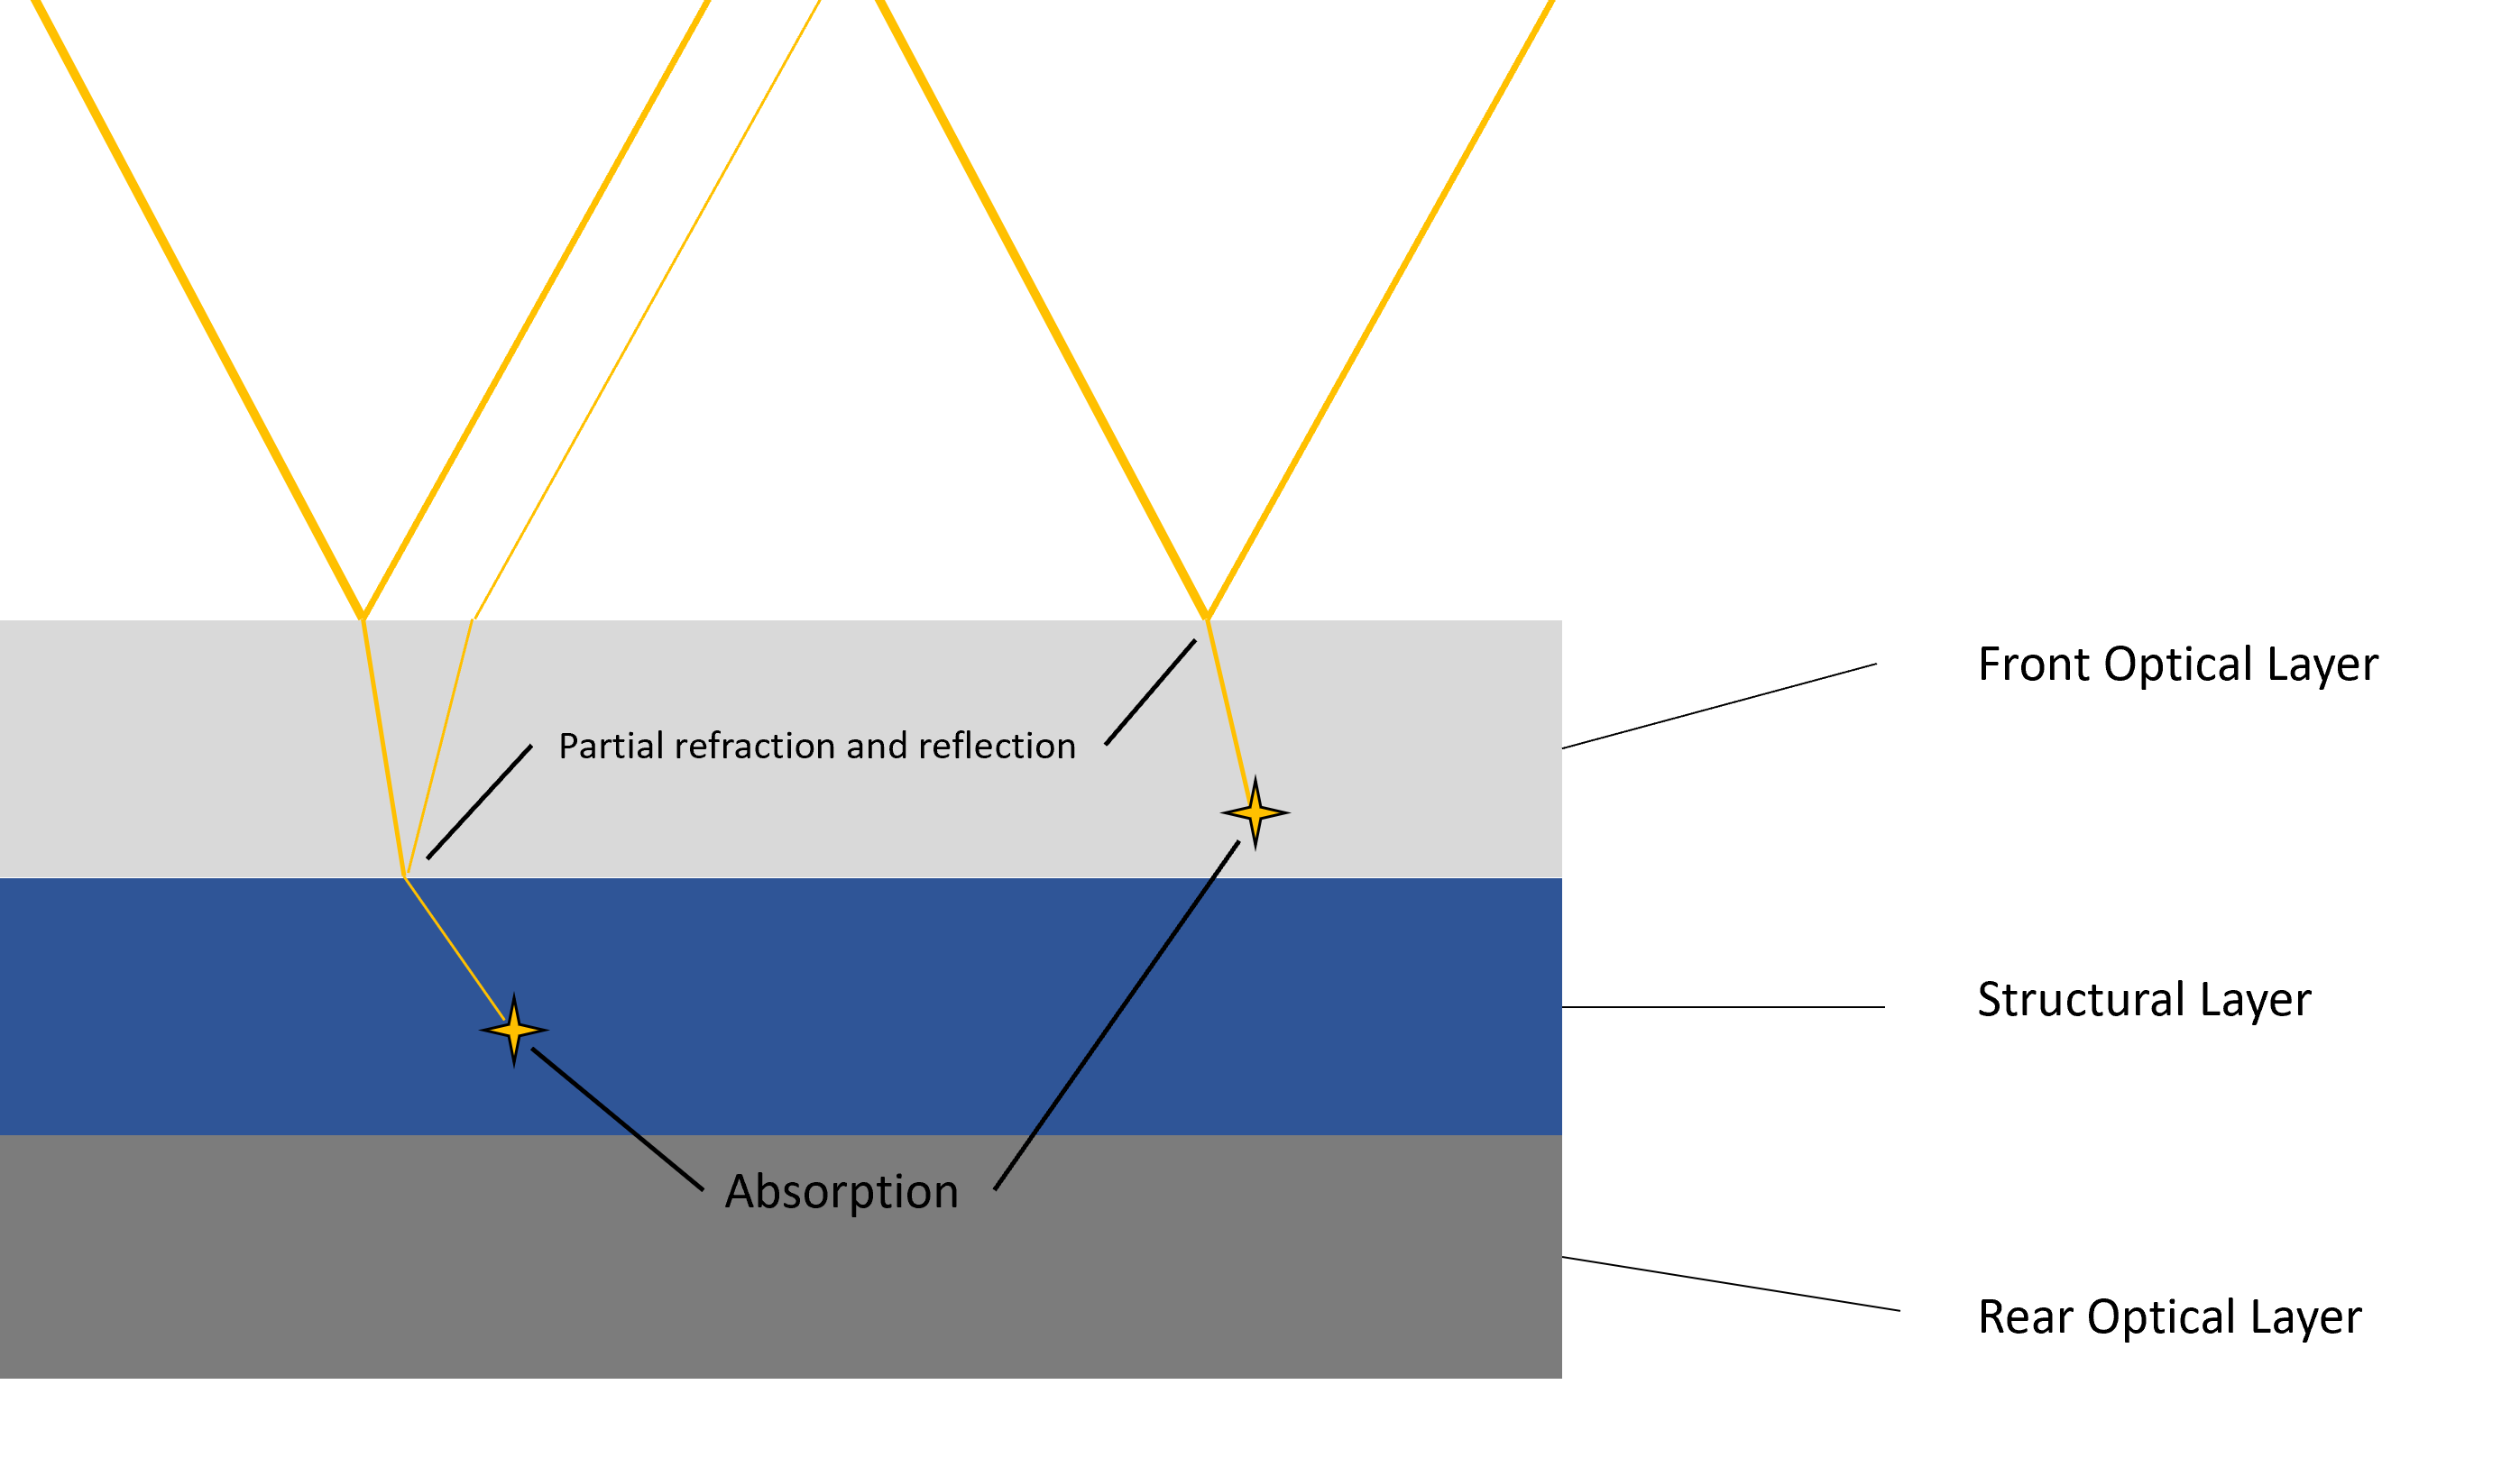
\includegraphics[width=14cm]{./resources/complicated_path.png}
  \caption{Example of paths the light hitting the sail could take}
  \label{fig:complicated_path}
\end{figure}

Figure \ref{fig:complicated_path} above shows two examples of how light might through the sail. The efficiency of a sail
will dependent on the rate of reflection to absorption and the direction of the emitted light. Furthermore, it is enough to look
at only the energies of the photons, as any other effects (i.e. polarization) are not relevant to the momentum transfer. Therefore
it needs to be examined how the light travels through the sail and how it is absorbed.
Three optical effects are important to determine this path:
\begin{enumerate}
  \item The refractive index at the different material interfaces, affecting the light path
  \item The percentage of light reflected (reflectivity)
  \item How likely it is for light to be absorbed given a distance traveled through the medium (absorption rate)
\end{enumerate}

Note that scattering within the material might also contribute to how the sail behaves. For simplicity its effect is
not looked at in this essay.

\subsection{Refraction}

To model refraction snell's law can be used with $n_1$ and $n_2$ being the refraction coefficients of the two materials
and $\theta_i$ and $\theta_t$ as the angle of incidence and transmission\autocite{Hecht2016-pd}:

\begin{equation}
  n_1 sin(\theta_i) = n_2 sin(\theta_t)
  \label{eq:snell}
\end{equation}

\subsection{Reflectivity}

Reflectivity describes how much of the light hitting a material gets reflected. This rate $R$ of reflected light is dependent on the incident angle $\theta_i$,
the angle of transmission $\theta_t$ and the polarization of
the incident light\autocite{Hecht2016-pd}. As for the material properties, the percentage is almost only dependent on the refraction coefficients
$n_1$ and $n_2$ of the two materials if the light is in the optical range\autocite{hoffman_driggers_2016}. The equations describing this behavior are called
the Fresnel equations, there is one for perpendicularly polarized light $R_p$ and for parallel polarized light $R_s$ (relative to the reflection surface, in this case the sail).
The equations look like this:

$$
R_s = \left| \frac{n_1 cos(\theta_i) - n_2 cos(\theta_t)}{n_1 cos(\theta_i) + n_2 cos(\theta_t)} \right|^2
    % = \left| \frac{n_1 cos(\theta_i) - n_2 \sqrt{1 - \frac{n_1}{n_2} sin(\theta_i)}}{n_1 cos(\theta_i) + n_2 \sqrt{1 - \frac{n_1}{n_2} sin(\theta_i)}} \right|^2
$$

$$
R_p = \left| \frac{n_1 cos(\theta_t) - n_2 cos(\theta_i)}{n_1 cos(\theta_t) + n_2 cos(\theta_i)} \right|^2
    % = \left| \frac{n_1 \sqrt{1 - \frac{n_1}{n_2} sin(\theta_i)} - n_2 cos(\theta_i)}{n_1 \sqrt{1 - \frac{n_1}{n_2} sin(\theta_i)} + n_2 cos(\theta_i)} \right|^2
$$

If the light is unpolarized both cases combine as there is an equal amount of both polarization components:

\begin{equation}
R = \frac{1}{2} (R_s+R_p)
\label{eq:reflecticity_unpolarized}
\end{equation}

Note that on refraction and reflection the relative amount of polarization might change. This can lead
to significantly more perpendicular or parallel polarized light, which in turns
has further effects on how the light behaves in the material.

\subsection{Rate of absorption}
When light travels through a material, it might get absorbed. To model the light sail it is important to find out what percentage of light get's
absorbed in a given distance $l$ traveled through the material. This value can be determined experimentally and is given through a constant
$\alpha$ which is called the absorption or extinction rate. 
% The US National Institute of Standards and Technology (NIST) provides publicly
% available data on this rate. They measure it as the mass absorption coefficient $\frac{\mu_a}{\rho_m}$. Where $\mu_a$ is the coefficient of
% absorption and $\rho_m$ the mass density. Therefore the mass absorption coefficient measures how much light is absorbed per a given amount
% of mass the light traveled through.\\
\\
The coefficient can be used together with the Beer Lambert law to determine how much the intensity of light drops for a given distance $l$:

\begin{equation}
  I = I_0 e^{- 4 \pi \alpha l / \lambda_0 }
  \label{eq:absorption}
\end{equation}


with $\lambda_0$ as the wavelength of the light to be absorbed.

\subsection{Thermals}

One additional challenge in a light sail are thermals. As the rate of absorption is somewhat constant and the rate of emission is dependent on the temperature
the sail will reach an equilibrium temperature $T$. This temperature within the capabilities of the materials chosen, otherwise they will melt, deform or
delaminate. At the same time it's not desireable to just increase the overall emissivity of the sail, as only light emitted in the right direction contributes.

\section{Examining a sail design}

\subsection{External conditions}

The characteristics of the light sail will be examined as if it where in Earth's orbit as that is the place where any light sail might be used first.
This means the light spectrum will be the Sun's with diminished intensity given by the Earth's distance to the Sun. Furthermore it means that the light
can be treated as being parallel as the distance to the light source is far enough. Finally no polarization effects need to be accounted for as the 
light from the Sun is unpolarized.\\
\\
The irradiance of the Sun at the distance of Earth is given by the solar constant:
$$
G_{SC} = 1.362 kW/m^2
$$
\\

It is roughly spread over the blackbody emission spectrum at the Sun's 
temperature (In reality, the irradiance differs slightly for specific wavelength due to absorption spectra).\\

Therefore Plank's blackbody radiation law can be used:
$$ 
B_{\lambda} = \frac{2 h c^2}{\lambda^5} \frac{1}{e^{h c / (\lambda k_B T)}-1}
$$

with $B_{\lambda}$ being the irradiance per square meter per wavelength per unit unit solid angle and $T$ as the temperature of the given body.

To analyze the efficiency of the sail, it is enough to know how the irradiance distributes over the spectrum. This can be achieved
by normalizing the blackbody radiation formula by the total energy emitted.
The total energy emitted is calculated by integrating over the spectrum:
$$
I = \int B_{\lambda} \,d \lambda
$$
The normalized blackbody radiation formula then looks like this:
$$
B_{\lambda n} = \frac{B_{\lambda}}{\int B_{\lambda} \,d \lambda}
$$


\subsection{The design of the sail}

The design that will be examined is Aluminized Mylar. A sail of this construction is proposed in a NASA document as a suitable
sail, given the suitability and availability of materials\autocite{hollerman}. The sail proposed in the paper would consist
of a structural layer made from $ 3 \mu m$ of mylar and a couting of $ 50 nm$ aluminum on each side. Mylar is a good choice
as a structural material, as it has high tensile strength and is very light. Aluminum is one of the best options as a
reflecting material, as its reflectivity is very high at almost all wavelength (further details can be found in the "Relevant Data"
section below). Note that as the back of the sail is made from aluminum as well no additional thrust is to be expected from emission, 
unless a temperature gradient develops within the sail.

\subsection{Relevant data}

Besides the natural constants, the only values needed for the analysis proposed above are the refractive index $n_{\lambda}$
and the absorption index $\alpha_{\lambda}$ at the relevant wavelength.\\
\\
Conveniently this data is openly available online at \hyperref{https://refractiveindex.info}{}{}{refractiveindex.info}\autocite{polyanskiy}.\\

\begin{figure}[H]
  \centering
  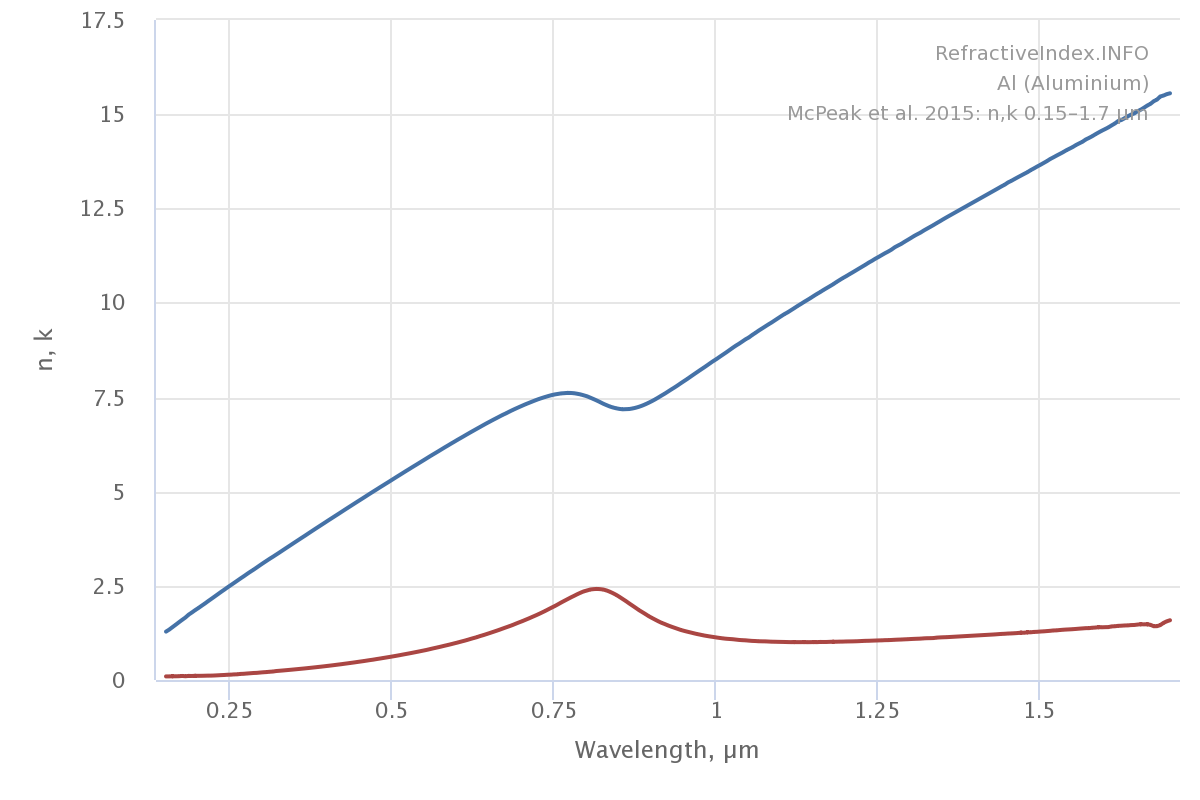
\includegraphics[width=12cm]{./resources/RefractiveIndexAl.png}
  \caption{Refractive index (n) and absorption constant (k) of Aluminum}
  \label{fig:complex_refraction_aliminum}
\end{figure}

\begin{figure}[H]
  \centering
  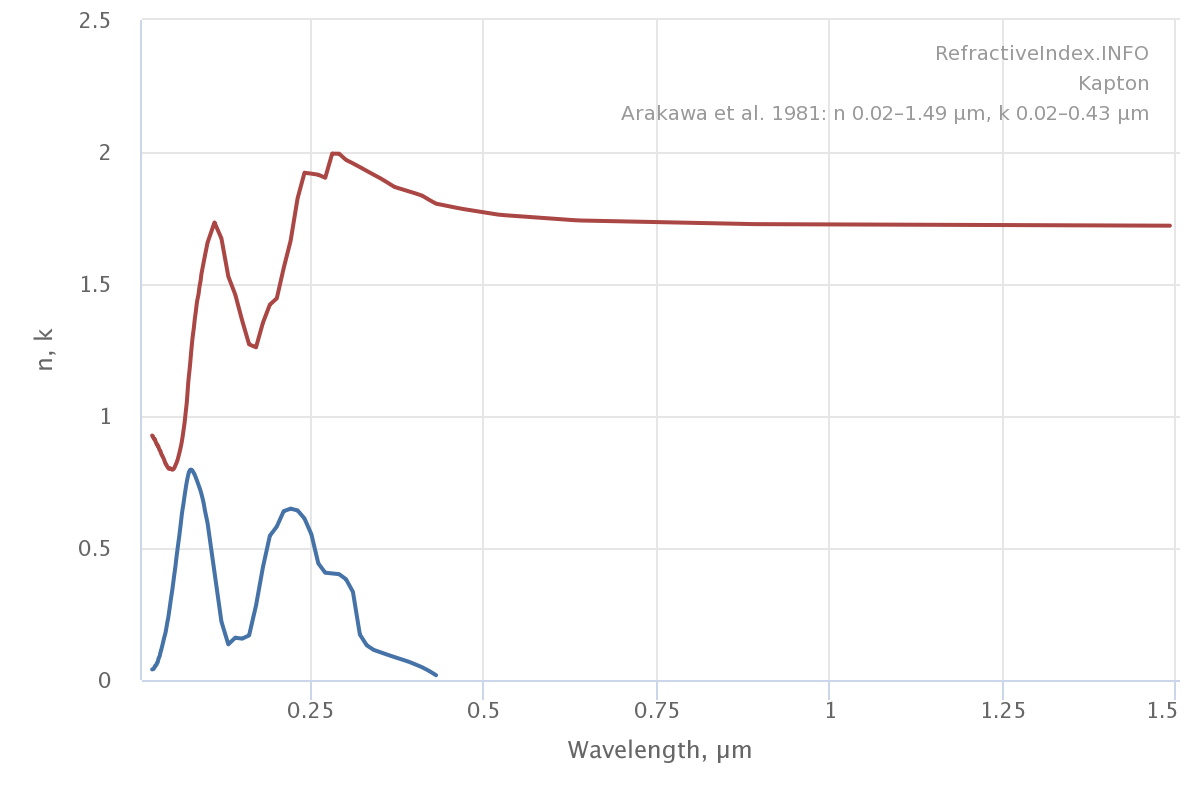
\includegraphics[width=12cm]{./resources/RefractiveIndexKapton.png}
  \caption{Refractive index (n) and absorption constant (k) of Kapton}
  \label{fig:complex_refraction_kapton}
\end{figure}

\begin{figure}[H]
  \centering
  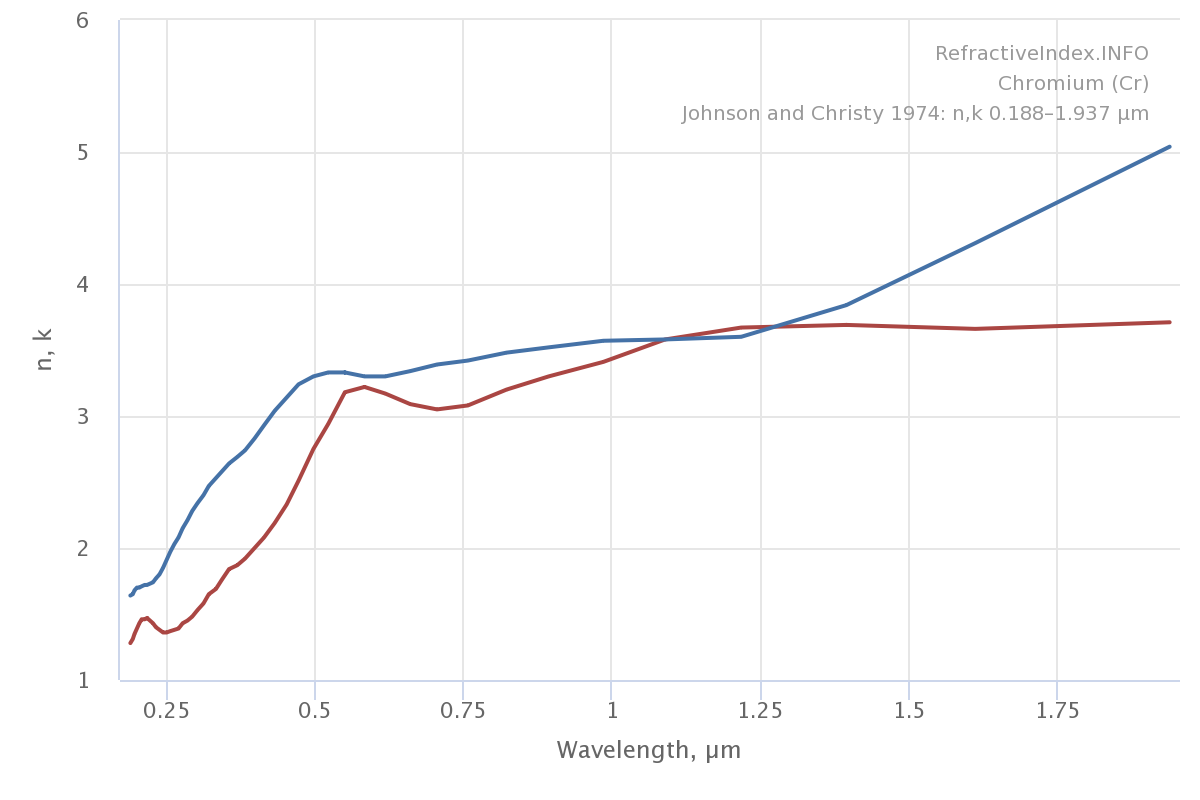
\includegraphics[width=12cm]{./resources/RefractiveIndexChrome.png}
  \caption{Refractive index (n) and absorption constant (k) of Chrome}
  \label{fig:complex_refraction_chrome}
\end{figure}

The website provides multiple datasets on each of the elements. For this analysis,
a dataset roughly in the range of the Sun's spectrum was chosen. Any values that
where missing, where interpolated or assumed to be the same as at the closest
available data point.

\subsection{Modelling the sail}

Analyzing what percentage of the light is reflected and absorbed by a given sail at a given angle and wavelength
is not easily done analytically. Therefore I created a new python simulation to achieve this based on the equations outlined
above. All python files can be either found online (\url{https://github.com/sidney-pauly/papers}) or attached to this document.

\subsubsection{Calculation of the absorbed and absorbed intensities at a given wavelength}
To determine how much light is reflected overall by the sail all possible paths suggested in figure \ref{fig:complicated_path}
have to be taken into account. The simulation program takes an iterative approach. The light is modeled as a uniform beam at a
specific wavelength and angle. For every material the beam passes through, it then determines how much of it is absorbed, how much
is reflected at the next interface and how much of it gets transmitted into the next material. The process is repeated
for the two resulting beams (reflected and transmitted beams) at the given reduced intensity. The initial intensity is normalized
to one for simpler analysis later\\
\\
The program first determines through trigonometry the path length taken through the material. This together
with the absorption constant $\alpha_{\lambda}$ (interpolated from the dataset given) can than be plugged into
equation \ref{eq:absorption} to determine how much light is left after traveling through the material.\\
\\
Next the percentage of reflected and absorbed light is calculated, this is done through formula \ref{eq:reflecticity_unpolarized}.
The relevant refractive indices $n_{\lambda}$ are again interpolated from the data set obtained from \hyperref{https://refractiveindex.info}{}{}{refractiveindex.info}\autocite{polyanskiy}.\\
\\
The process is repeated for the two resulting beams as long as the intensity is high enough. If there is no next material, this
corresponds to the light exiting the material and it is added to the total reflected intensity.\\

\begin{figure}[H]
  \centering
  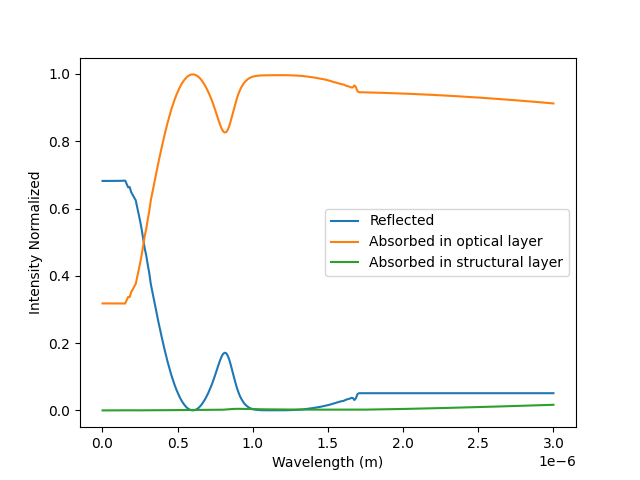
\includegraphics[width=14cm]{./python/output/reflection_and_absorption_aluminum_sail.png}
  \caption{Relative intensity of the absorbed and reflected light hitting the proposed sail}
  \label{fig:aluminum_sail}
\end{figure}

The process can then be repeated for different wavelength which leads to the output above (figure \ref{fig:aluminum_sail})

\subsubsection{Analysing the resulting efficiency}

\begin{figure}[H]
  \centering
  \includegraphics[width=14cm]{./python/output/blackbody_radiation_Sun.png}
  \caption{Normalized and idealized spectrum of the Sun}
  \label{fig:spectrum_Sun}
\end{figure}

These intensities now have to be related to the wavelength given off by the Sun. Figure \ref{fig:spectrum_Sun} above
shows the idealized (no absorption and emission lines) and normalized (combined intensity, i.e. area under the graph of one). As both
the absorption/reflection intensities of the sail and the Sun's light spectrum are given in a normalized form
they can simply be multiplied to give the weighted intensity of reflected and absorbed light energy:

\begin{figure}[H]
  \centering
  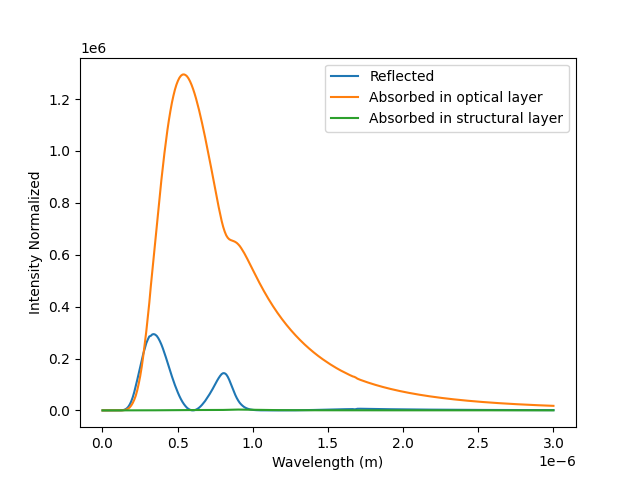
\includegraphics[width=14cm]{./python/output/reflection_and_absorption_aluminum_sail_weighted.png}
  \caption{Relative intensity of the absorbed and reflected light weighted by the amount of light at the given wavelength}
  \label{fig:aluminum_sail_weighted}
\end{figure}

Integrating over each of the curves will result in the normalized overall energy per unit area absorbed or reflected.
These two quantities will be called $I_{a}$ and $I_{r}$ respectively\\
Recalling formula \ref{eq:light_force} and the fact that the force doubles if light is reflected we can derive the following 
formula for the overall force per area ($A$). Note that this is the force 
perpendicular to the sail $F_{\perp}$. 

$$
  \frac{F_{\perp}}{A} = \frac{ 2 cos(\theta) I_{r} + cos(\theta) I_{a} }{c}
  = cos(\theta) \frac{ 2  I_{r} + I_{a} }{c}
$$

Any light absorbed will also contribute to a force at a direction parallel to the sail's surface $F_{\parallel}$:

$$
  \frac{F_{\parallel}}{A} = \frac{ sin(\theta) I_{a} }{c}
$$

Note that $cos(\theta)$ are added as the any force applied perpendicular to the sails
decrease with an increasing angle of attack. inversely $sin(\theta)$ is added as the
force parallel to the sail increases with an increasing angle of attack.
 
The combined force will therefore be given by:

$$
\frac{F}{A} = \sqrt{F_{\parallel}^2 + F_{\perp}^2}
$$

From this, the efficiency of the sail can now be calculate. A 100\% efficient sail
would be one that reflects 100\% of the light that hits it. The resulting force
will be called $F_{max}$. This is because reflected
light leads to twice the force, therefore this is the most efficient setup\footnote{
  A sail that absorbed all the radiation and then emits all of it directionally would 
  be as efficient
}. \\
Note that as we are dealing with the force per unit area it has to be considered that the area
of the sail actually facing the Sun reduces as the sail is rotated. This factor
will not be factored into the following efficiency. This has the benefit of enabling
a pure analysis of just the optical characteristics of the sail. As a result this efficiency
will be coined optical efficiency in this essay and will be denoted by $\epsilon_{o}$.
The actual efficiency can be easily obtained by multiplying this efficiency with $cos(\theta)$ as the
available area facing the sun decreases with that factor.

$$
\epsilon_{o} = \frac{\sqrt{F_{\parallel}^2 + F_{\perp}^2}}{F_{max}} 
= \frac{\sqrt{(cos(\theta) \frac{ 2  I_{r} + I_{a} }{c})^2 + (\frac{ sin(\theta) I_{a} }{c})^2}}{\frac{2 I_s}{c}}
$$

with $I_s$ as the irradiance of the light source.

$$
\epsilon = cos(\theta) \epsilon_{o}
$$

Plotting the optical efficiency leads to the following graph:

\begin{figure}[H]
  \centering
  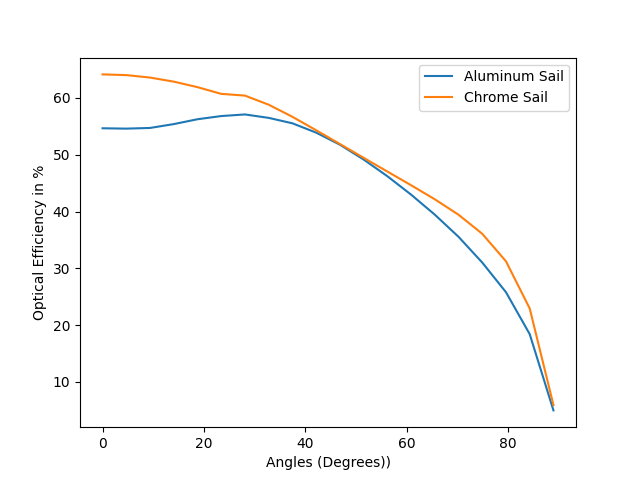
\includegraphics[width=12cm]{./python/output/optical_efficiency.png}
  \caption{The optical efficiency of two light sails $\epsilon_{0}$ at different angles $\theta$}
  \label{fig:optical_efficiency}
\end{figure}

Note that this graph includes a second light sail. It is identical to the first light sail except that the front
optical layer has been swapped for chromium.\\
\\
The actual efficiencies of the two sails look like this:

\begin{figure}[H]
  \centering
  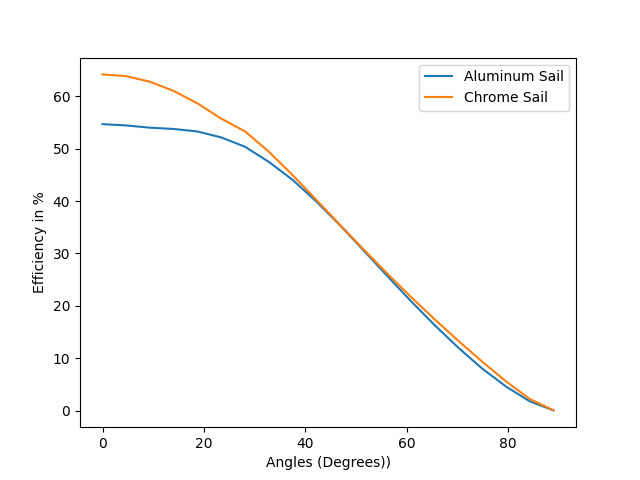
\includegraphics[width=12cm]{./python/output/efficiency.png}
  \caption{The efficiency of two light sails $\epsilon$ at different angles $\theta$}
  \label{fig:efficiency}
\end{figure}

\section{Discussion}
From the obtained data quite a few things about light sails and there makeup become apparent. First and foremost
it could be shown that the front optical layer of a light sail makes a significant impact on it's efficiency (10\% difference
for chrome vs. aluminum). In the making of any light sail the properties of the front optical layer should therefore be analyzed thoroughly.
Any material that can give a higher reflectivity in the important spectrum will perform a lot better. The aluminum
that was analyzed seems to be suboptimal, as it performs badly in in the range of the important wavelength
given the Sun's spectrum (see figure \ref{fig:aluminum_sail}). When considering to swap the aluminum for a different
material or when improving the aluminum used the focus should be on boosting the reflectivity in that range.\\
\\
Furthermore in the shown model a lot of the light hitting the sail is not reflected. Most of it gets transmitted
into the first optical layer. As the reflection of light is so important to a sails efficiency it should be considered
if the reflectivity could be boosted through additional optical layers. Putting a different material in front of
the aluminum might for example lead to total internal reflection which could help a lot with the reflectivity,
especially at greater angles of the sail to the light source.\\
\\
In the shown example it was assumed that the sail would radiate it's heat away in all directions uniformly. However
given the high rate of absorption, emitting radiation directionally would help a lot with efficiency. Supporting 
directional emission, is the fact that most of the light seems to get absorbed in the first optical layer, rather
than in the structural layer. This means that if the structural layer is sufficiently isolating, a temperature gradient
could be achieved. This would mean the light would mostly get emitted from the hot side (the first optical layer),
and therefore directional emission would generate additional thrust.\\
\\
Considering the proposed model, the orientation of the sail relative to the light source, does not seem to be that important 
to the sails efficiency (The efficiency only starts to drop significantly with more then 10 degrees of variation).
This is probably due to the fact that the emitted force is still quite effective as the angle
increases. For actual operation of a light sail this is good news, as it allows for greater navigational freedom. 

\section{Limitations}

Analyzing light sails with this method seams to give promising results. The resulting efficiencies seem
to be plausible and in a range where the light sails would be actually usable for space travel. However the
computational model is build on top of theoretical assumptions and is not considering the full extend
of all physical effects light could have on the sail. While experimental data of any optical structure
that can be simulated with the model would be ideal to verify it, there are also some theoretical limitations
that should be considered.

\subsection{Polarization}
As mentioned, currently the polarization of the light is not taken into account. Polarization of the light
after the first transmission into the medium could have considerable effects on the amount of reflected
or absorbed light. Extending the model with polarization should be a straight forward extension to the
current model and could be considered in future iterations.

\subsection{Dispersion}
Dispersion is currently not modeled. Dispersion could have an effect as it would introduce light
beams traveling at different angles. It is likely that this would degrade efficiency rather than
boost it as rays traveling at an angle have a higher likelihood of being absorbed (greater distance traveled).
Compounding to this, is that dispersed rays would likely be deflected away from the sail at a greater angle as
the incidence ones this would decrease the momentum transfer.

\subsection{Thin layer effects}
As the layers of the sail are roughly in the same range as the wavelength of the light additional physical
effects could come into play. The relevant phenomena would need to be investigated

\subsection{Heating}
The current model does not simulate the material heating up and emitting radiation. As such a simulation
would be completely independent from any optical behavior of the sail it would be best to create a separate model
to investigate these effects.

\printbibliography

\end{document}
